\section{Prototyping}


Prototypes develop from sketches over time and are more defined in their criteria weights. 
Make multiple protopytes to evaluate different approaches and check for failure/success. Prototypes help us uderstand requirements and specifications of the idea.
They answer a specific question. \medskip

\textit{Vertical vs. horizontal}
Vertical provides critical path of one or few features (real feature on that path is completed). Horizontal provides only overview with little to no functionality. \medskip

\textit{Fidelity and Interactivity}

\begin{center}
	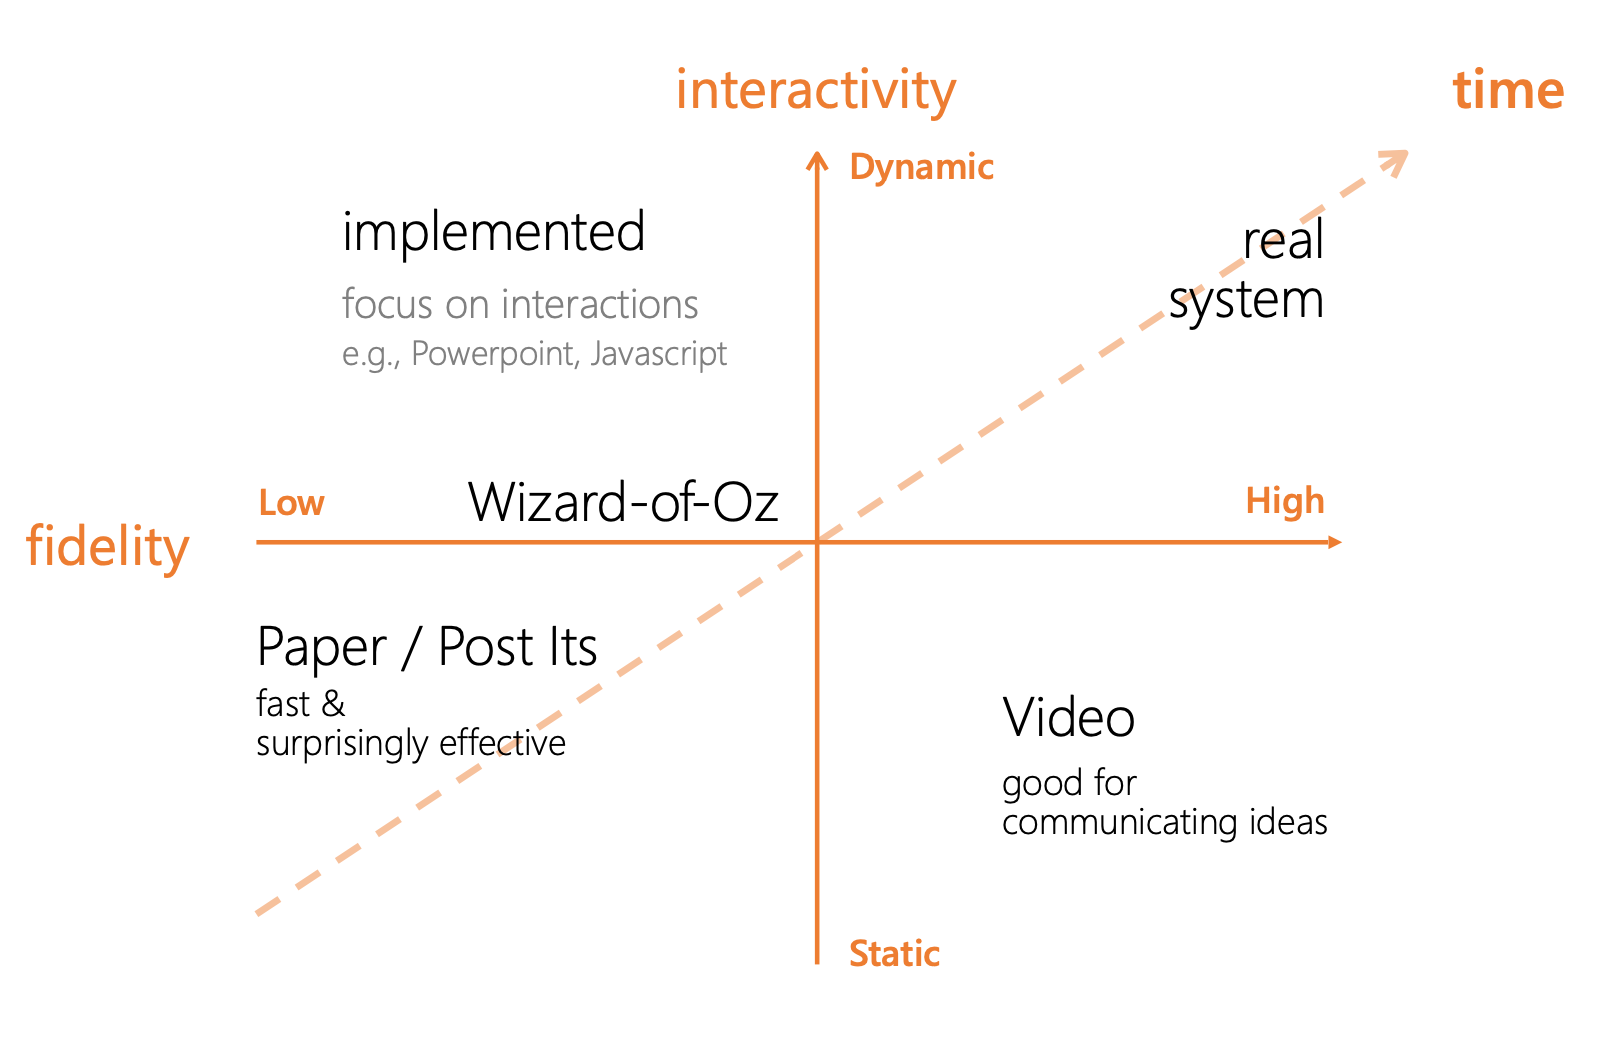
\includegraphics[width=\linewidth]{fidelity_iteractivity.png}
\end{center}


\textbf{Paper prototypes}
Are rapid and cheap. \medskip

\textbf{Wizard of Oz}
Interprets user input and simulated a system response. Allowd rapid testing of complex feature before implementing. \medskip

\textbf{MidFi-Prototypes}

Physical (paper, cardboard, lego etc.) to software. \medskip

\begin{multicols}{2}
    \begin{itemize}[itemsep=-5pt, topsep=-20pt, leftmargin=*]
	\item Powerpoint, Keynote
	\item AdobeXD, Figma
	\end{itemize}
\end{multicols}



\begin{center}
	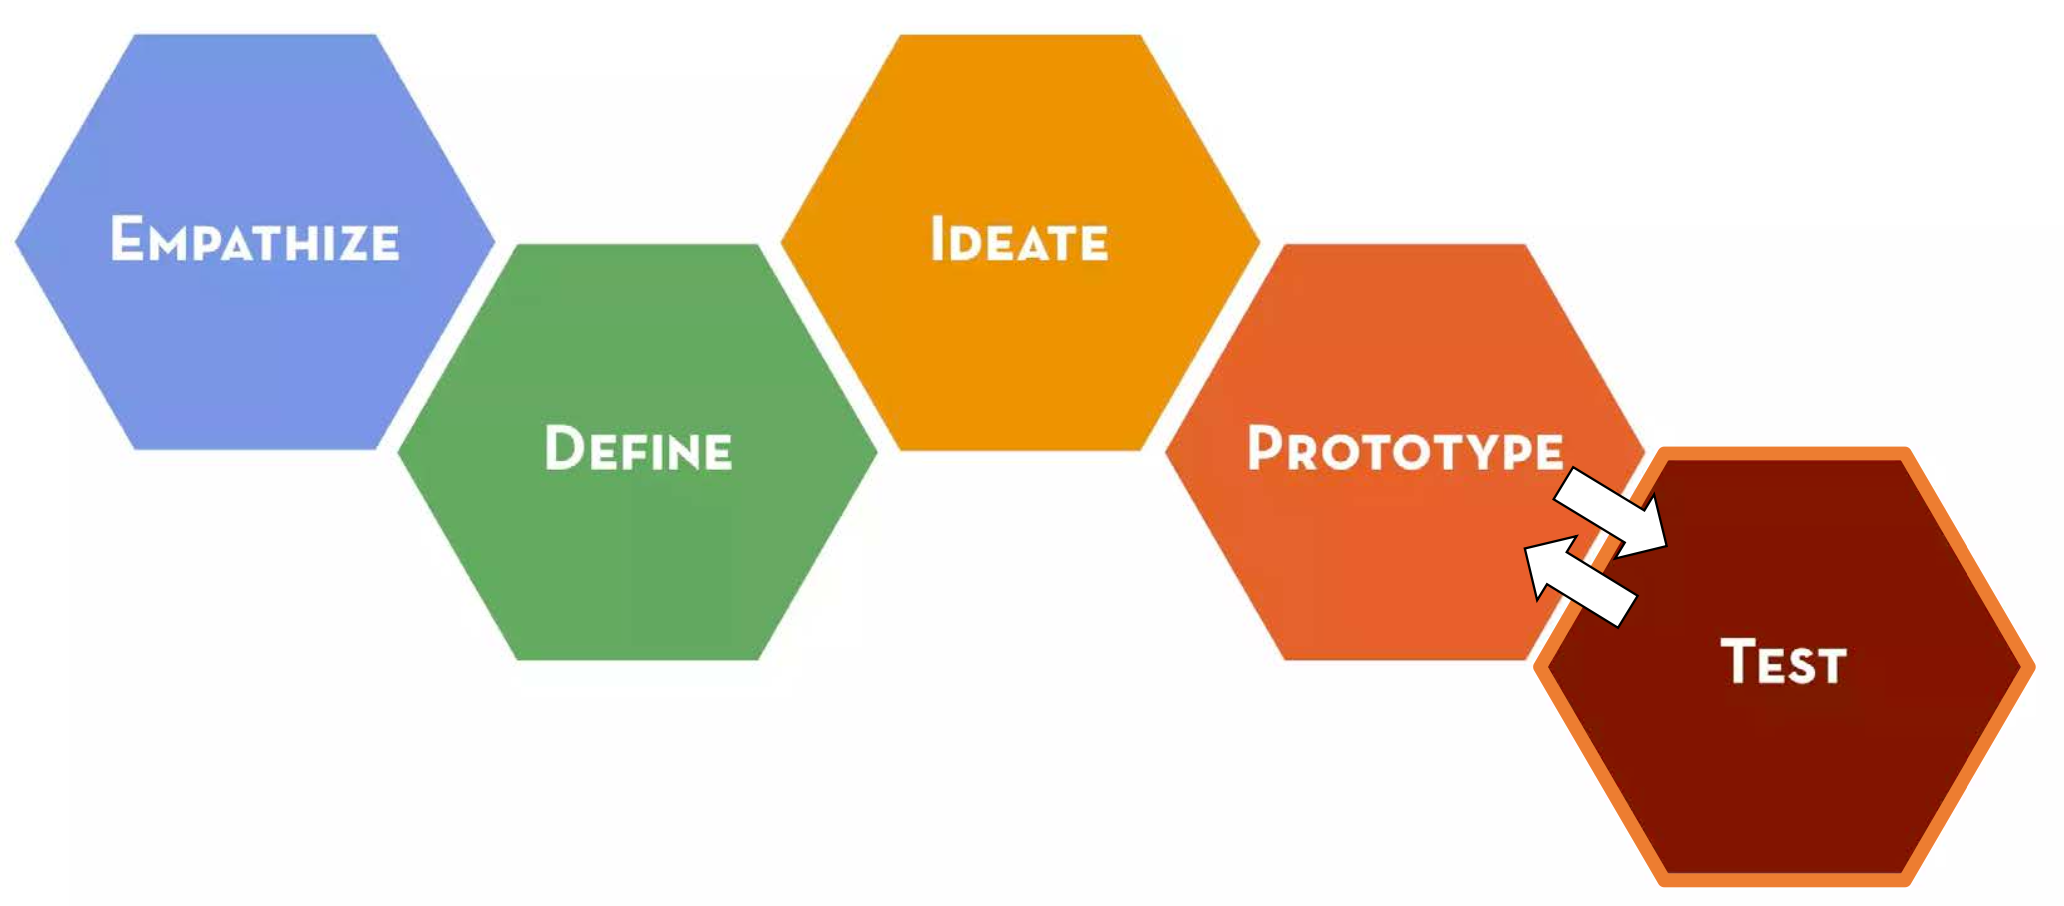
\includegraphics[width=\linewidth]{prototype_test.png}
\end{center}


\textbf{Anylytical vs. Empirical} \smallskip

\textit{Analytical} \smallskip

Look at inherent attributes of the design, rather then the desing in use. Intrinsic characteristics of the design. 
Examples are usability/UX inspection methods, design walkthroughs, heuristic evaluations. \medskip

\textit{Empirical} \smallskip

Based on how well a design or design change pays off in terms of real observable usage. Includes quantitative and qualitative data. 
Examples are usability/UX scores, controlled experiments and case studies. 

\textbf{Formative vs. Sumative} \smallskip

\textit{Formative} \smallskip

Helps form the design. Part of iterative process. Evaluations done during testing. Mainly collects qualitative data but also quantitative. Focusses on what is not working.\smallskip

\textit{Summative} \smallskip

Helps sum up the design. Evaluates the success of the finished product, and compares with competitors. Collects quantitative data, and focussed mainly on what is working. \medskip


\textbf{Evaluation criteria for UI design} \smallskip

\textit{Usability} \smallskip

Extent to which product can be used by specific users to achieve goals with effectiveness, efficiency and satisfaction.

Five quality components of Usability:

\begin{multicols}{2}
    \begin{itemize}[itemsep=-5pt, topsep=-20pt, leftmargin=*]
	\item learnability
	\item efficiency
	\item memorability
	\item errors
	\item satisfaction
	\end{itemize}
\end{multicols}

\textit{User Experience} \smallskip

Totality of the effect(s) felt by a user as a result of interaction with the usage context of a system. device or product. 

It includes:  
\begin{multicols}{2}
    \begin{itemize}[itemsep=-5pt, topsep=-20pt, leftmargin=*]
	\item Usability
	\item usefulness
	\item emotional impact
	\item savoring memory after interaction
	\end{itemize}
\end{multicols}
It embraces seeing, touching, thinking about system or product and admiring it and its presentation.
Focusses on holistic experience of user. \medskip


\textbf{Affordances}
Actions that the design of an obkect suggest to the user. Provide strong clues to how objects are to be used without labels, explanations or manuals. \smallskip

Works for both physical objects and software. Up to a certain degree of complexity. 